\section{De RNN's a Transformers}

Las Redes Neuronales Recurrentes o RNN (por sus siglas en Inglés) datan del año 1986, basadas en el
trabajo de Rumelhart \cite{Rumelhart}. Este tipo de redes están especializadas en el procesamiento
de datos que contienen información temporal, mejorando los resultados obtenidos por por otros tipos
de redes como Redes FeedForward o Redes Convolucionales.

La principal idea detrás de estos modelos de red es el concepto de \textit{Parameter Sharing}.
Con \textit{Parameter Sharing} un modelo un modelo puede generalizar mejor cuando la información
que esta contenida en diferentes partes de una secuencia. Así, el modelo no necesita aprender
independientemente todas las reglas que forman la secuencias, sino que ahora, la salida para cada
elemento en el tiempo esta determinada por la salida del elemento anterior. Resultando en una
recurrencia con las mismas reglas de actualización aplicadas a cada elemento en el tiempo.
La ecuación \ref{eq:rnn} representa este proceso; $h^{(t)}$ es el estado de la recurrencia aplicada
por alguna función $f$ a un elemento $x^{(t)}t$ de la secuencia $x$ en el tiempo, $t$ y $\theta$ son
los parámetros compartidos.

\begin{equation}
    h^{(t)} = f(h^{(t-1)}, x^{(t)}; \theta)
\end{equation}
\label{eq:rnn}

En una RNN vista como un gráfo computacional dirigído y acíclico, cada nodo representa un estado en
la recurrencia y procesa la información de la secuencia $x$ con los mismos parámetros $\theta$ en cada
paso, observe la figura \ref{fig:rnn_cg}.

\begin{figure}[h!]
\centering
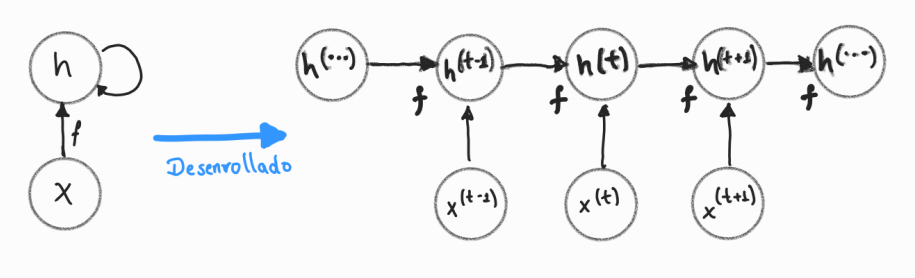
\includegraphics[width=.8\textwidth]{Chapters/1. Transformer/Figures/rnn/rnn_cgraph.png}
\caption[RNN - Grafo Computacional]{Grafo computacional generado por una RNN al "desenrrollar" la
recurrencia. Usando los parámetros compartidos en cada nodo, con cada elemento $x^{(t)}$ de la
secuencia genera un nuevo estado oculto $h^{(t)}$ para retroalimentar nuevamente la entrada del
siguiente nodo.}
% the \label gives a reference for this figure so that you can refer to it in the text by its number in a way which will be automatically updated if you change the document.  THIS IS A GOOD IDEA; having automatically updated references for figures, equations, etc, will keep your document in order even as you continue to update it over a period of months.  This reference can be called in the text using the \ref tag.
\label{fig:rnn_cg}
\end{figure}

Existen diversas formas como construir Redes neuronales Recurrentes; pueden producir una
salida en cada paso de tiempo o tener solo una al final de la recurrencia  y también pueden tener
conexiones entre unidades ocultas. La manera más común de es la ilustrada en la figura
\ref{fig:rnn_cfg}a. Cada etapa de la recurrencia es retroalimentada por la activación del estado oculto
previo. Así, $h^{t}$ contiene información codificada de elementos previos de la secuencia que puede
ser usada en el futuro para obtener una salida $O^{(t+1)}$. En la figura \ref{fig:rnn_cfg}b se
cambia la retroalimentación de $h^{(t)}$ por $O^{(t)}$. Nótese que en este caso, la red es entrenada
para obtener un valor en específico $O^{(t)}$ lo que provocaría que gran parte de la información de
los estados ocultos pasados $h^{(t-1)}, h^{(t-2)}, ...$ no se transmita. En el esquema anterior
\ref{fig:rnn_cfg}a la red es entrenada para decidir que información transmitir en el futuro a través
de los estados ocultos, y en la figura \ref{fig:rnn_cfg}b cada estado esta conectado con el pasado
a través de la predicción del paso anterior, perdiendo gran parte de la información a menos que
la salida $O^{(t-1)}$ sea lo suficientemente rica al estar en altas dimensiones.

\begin{figure}[h!]
\centering
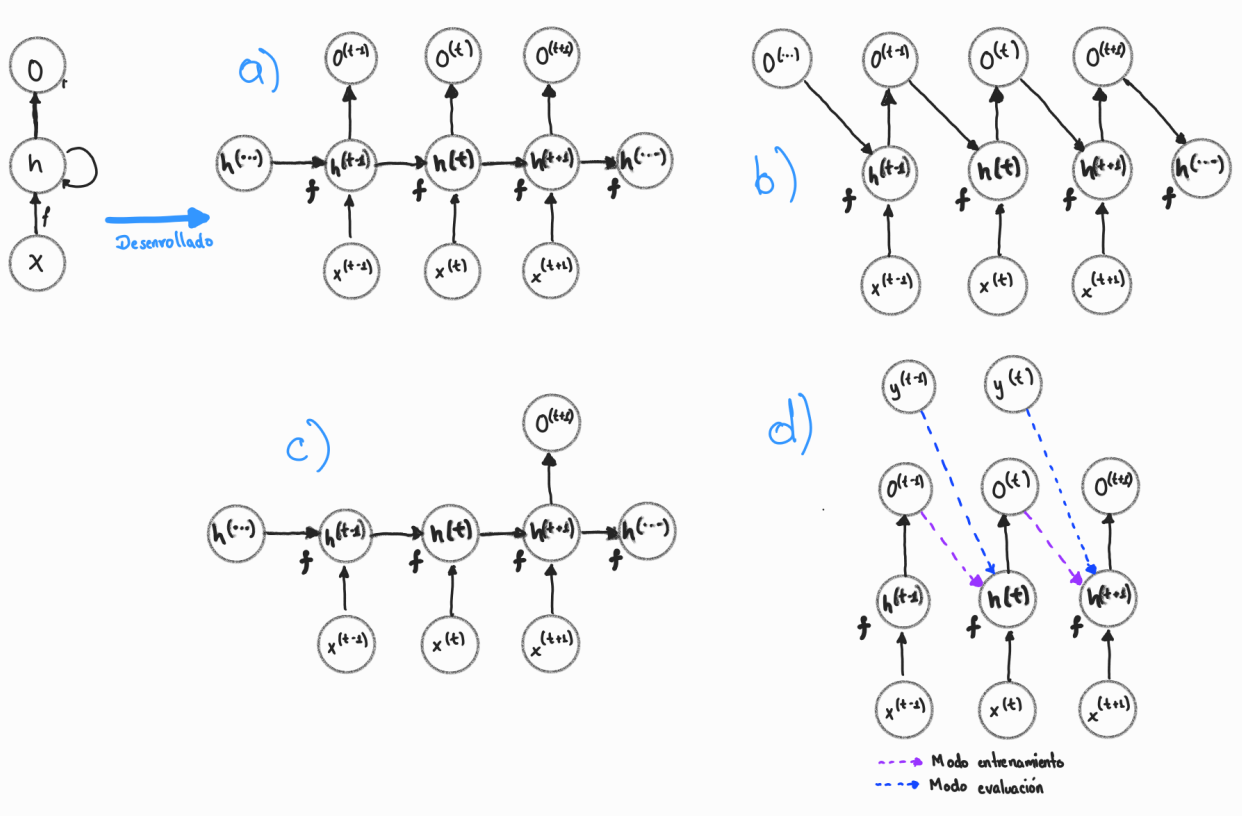
\includegraphics[width=.8\textwidth]{Chapters/1. Transformer/Figures/rnn/rnn_cfg.png}
\caption[RNN - CFG]{Distintos tipos de RNNs. \textbf{a)} Las activaciones de las capas ocultas $h^{(t)}$
alimentan al nodo siguiente, cada etapa de la recurrencia genera una salida $O^{(t)}$ \textbf{b)}
Cada nodo es alimentado por las salidas de cada estado oculto $O^{(t)}$. \textbf{c)} Solo tiene una
salida $O^{(t)}$ al final de la recurrencia, puede ser usada para resumir/predecir un valor de una
secuencia. \textbf{d)} Teacher Forcing.}
% the \label gives a reference for this figure so that you can refer to it in the text by its number in a way which will be automatically updated if you change the document.  THIS IS A GOOD IDEA; having automatically updated references for figures, equations, etc, will keep your document in order even as you continue to update it over a period of months.  This reference can be called in the text using the \ref tag.
\label{fig:rnn_cfg}
\end{figure}


La RNN representada en la figura \ref{fig:rnn_cfg}c tiene una sola salida al final de la
recurrencia. Al contrario de las anteriores, este tipo de redes pueden ser usadas para resumir
información contenida en la secuencia para predecir un único valor final. El Análisis de Sentimiento
en textos es una tarea común que puede ser representada con este esquema de red.

- Hablar de Teacher forcing como parte de una comparativa
    - Mencionar parallización y backpropragation trougth the time
- Hablar de modelo de página 381
- Mencionar bidirecionalidad pag 383

- Celdas de memoria LSTM GRU
- Problema de RNN
Vanising gradient
https://www.iro.umontreal.ca/~lisa/pointeurs/ieeetrnn94.pdf
https://arxiv.org/pdf/1211.5063.pdf

- Attention mechanism



\section{El modelo Transformer}

A finales del año 2017 se presentó un nuevo modelo que vino a revolucionar el área de Procesamiento
de Lenguaje Natural, El Transformer \cite{Vaswani}. Una de sus principales características es la
capacidad de procesar la información de alguna secuencia de forma paralela, caso contrario a las
Redes Neuronales Recurrentes, donde la información se procesa recurrentemente. Gracias a ello
la capacidad de \textit{recuerdo} no se ve afectado por el problema de \textit{El
desvanecimiento del Gradiente} cuando se trabaja con secuencias bastante largas.
